\documentclass[border=2mm]{standalone}
\usepackage{tikz}
\usetikzlibrary{intersections}
\begin{document}



\begin{tikzpicture}
\clip (-2,-2) rectangle (2,2);
\draw [name path=curve 1] (-2,-1) .. controls (8,-1) and (-8,1) .. (2,1);
\draw [name path=curve 2] (-1,-2) .. controls (-1,8) and (1,-8) .. (1,2);
\fill [name intersections={of=curve 1 and curve 2}]
(intersections-1) circle (2pt)
(intersections-2) circle (2pt);
\end{tikzpicture}


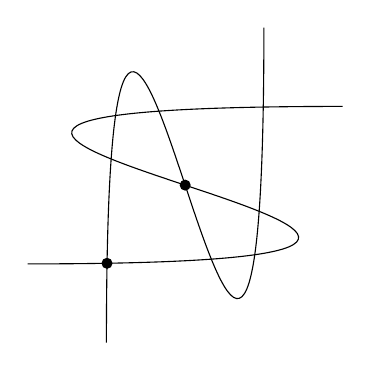
\begin{tikzpicture}
\clip (-2,-2) rectangle (2,2);
\draw [name path=curve 1] (-2,-1) .. controls (8,-1) and (-8,1) .. (2,1);
\draw [name path=curve 2] (-1,-2) .. controls (-1,8) and (1,-8) .. (1,2);
\fill [name intersections={of=curve 1 and curve 2, by={a,b}}]
(a) circle (2pt)
(b) circle (2pt);
\end{tikzpicture}





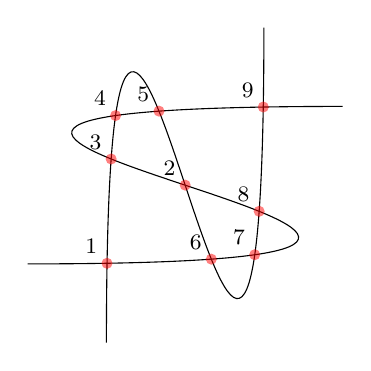
\begin{tikzpicture}
\clip (-2,-2) rectangle (2,2);
\draw [name path=curve 1] (-2,-1) .. controls (8,-1) and (-8,1) .. (2,1);
\draw [name path=curve 2] (-1,-2) .. controls (-1,8) and (1,-8) .. (1,2);
\fill [name intersections={of=curve 1 and curve 2, name=i, total=\t}]
[red, opacity=0.5, every node/.style={above left, black, opacity=1}]
\foreach \s in {1,...,\t}{(i-\s) circle (2pt) node {\footnotesize\s}};
\end{tikzpicture}

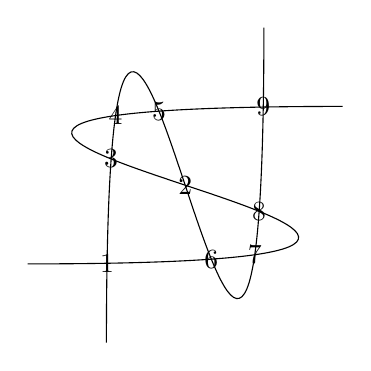
\begin{tikzpicture}
\clip (-2,-2) rectangle (2,2);
\draw [name path=curve 1] (-2,-1) .. controls (8,-1) and (-8,1) .. (2,1);
\draw [name path=curve 2] (-1,-2) .. controls (-1,8) and (1,-8) .. (1,2);
\fill [name intersections={
of=curve 1 and curve 2, total=\i,
by={[label=center:1],[label=center:...],[label=center:\i]}}];
\end{tikzpicture}


 
 
\end{document}